%\iffalse meta-comment
%Copyright (c) 2020 Peter Rowlett
%
%Permission is hereby granted, free of charge, to any person obtaining a copy
%of this software and associated documentation files (the "Software"), to deal
%in the Software without restriction, including without limitation the rights
%to use, copy, modify, merge, publish, distribute, sublicense, and/or sell
%copies of the Software, and to permit persons to whom the Software is
%furnished to do so, subject to the following conditions:
%
%The above copyright notice and this permission notice shall be included in all
%copies or substantial portions of the Software.
%
%THE SOFTWARE IS PROVIDED "AS IS", WITHOUT WARRANTY OF ANY KIND, EXPRESS OR
%IMPLIED, INCLUDING BUT NOT LIMITED TO THE WARRANTIES OF MERCHANTABILITY,
%FITNESS FOR A PARTICULAR PURPOSE AND NONINFRINGEMENT. IN NO EVENT SHALL THE
%AUTHORS OR COPYRIGHT HOLDERS BE LIABLE FOR ANY CLAIM, DAMAGES OR OTHER
%LIABILITY, WHETHER IN AN ACTION OF CONTRACT, TORT OR OTHERWISE, ARISING FROM,
%OUT OF OR IN CONNECTION WITH THE SOFTWARE OR THE USE OR OTHER DEALINGS IN THE
%SOFTWARE.
%\fi
%\section{Background}
%
%\lstinline{nimsticks} is a package for \LaTeX{} that draws sticks for representating games of Nim. 
%
%The idea is that just drawing a Nim game like IIIII looks visually uninteresting because it is too regular. Instead, this uses \lstinline{tikz} to draw sticks and \lstinline{lcg} for random numbers to offset the top and bottom of each stick, so it looks less regular.
%
%It does this by providing two commands: 
%\begin{itemize}
%\item \lstinline{\drawnimstick}: draws a single Nim stick with a little random wobble;
%\item \lstinline{\nimgame}: takes a comma-separated list of numbers and draws a line of Nim heaps holding those number of sticks.
%\end{itemize}
%
%\section{Usage}
%
%For example, the input \lstinline!\nimgame{3,5,4}! will produce output like this (precise look affected by random wobble in the sticks):
%
%\nimgame{5,3,4}
%
%It is likely the user will want to use \lstinline{\nimgame} and not \lstinline{\drawnimstick} directly, but the input \lstinline{\drawnimstick} will produce output like this (precise look affected by random wobble in the sticks): \drawnimstick
%
%\lstinline{\nimgame} will happily work with one heap, so the input \lstinline!\nimgame{7}! will produce output like this (precise look affected by random wobble in the sticks):
%
%\nimgame{7}
%
%\section{Issues}
%
%In principle, if you add lots of piles it will just wrap onto multiple lines, though it will start to look less clear. For example, the input\\
%\lstinline!\nimgame{1,2,3,4,5,6,7,8,9,10,9,8,7,6,5,4,3,2,1}!\\
%will produce the output:
%\nimgame{1,2,3,4,5,6,7,8,9,10,9,8,7,6,5,4,3,2,1}
%Similarly, if you have a lot of sticks in the same heap, it will wrap and look confusing, for example the input \lstinline!\nimgame{128}! will produce the output:
%\nimgame{256}
%\iffalse
%<*documentation>
\documentclass{article}
\usepackage{nimsticks}
\usepackage{doc}
\usepackage{listings}
\lstset{basicstyle=\ttfamily\footnotesize,commentstyle=\color{white},language=TeX}
\title{nimsticks}
\author{Peter Rowlett}
\begin{document}
\maketitle
    \DocInput{nimsticks.dtx}
\end{document}
%</documentation>
%\fi

%\iffalse
%<*nimsticks>
\ProvidesPackage{nimsticks}[2020/07/12 nimsticks 1.0]
\RequirePackage[first=-100,last=100,seed=0]{lcg}
\RequirePackage{tikz}
\@ifundefined{drawnimstick}{}
    {\PackageWarning{nimsticks}{Command `drawnimstick' already defined}}
\@ifundefined{nimgame}{}
    {\PackageWarning{nimsticks}{Command `nimgame' already defined}}
\@ifundefined{listofgames}{}
    {\PackageWarning{nimsticks}{Command `listofgames' already defined}}
\@ifundefined{c@topx}{}
    {\PackageWarning{nimsticks}{Counter `topx' already defined}}
\@ifundefined{topx}{}
    {\PackageWarning{nimsticks}{Existing command `topx' conflicts with counter `topx'}}
\@ifundefined{c@botx}{}
    {\PackageWarning{nimsticks}{Counter `botx' already defined}}
\@ifundefined{botx}{}
    {\PackageWarning{nimsticks}{Existing command `botx' conflicts with counter `botx'}}
\@ifundefined{c@heap}{}
    {\PackageWarning{nimsticks}{Counter `heap' already defined}}
\@ifundefined{heap}{}
    {\PackageWarning{nimsticks}{Existing command `heap' conflicts with counter `heap'}}
\@ifundefined{c@heapindex}{}
    {\PackageWarning{nimsticks}{Counter `heapindex' already defined}}
\@ifundefined{heapindex}{}
    {\PackageWarning{nimsticks}{Existing command `heapindex' conflicts with counter `heapindex'}}
\newcommand{\drawnimstick}{%
    \rand\pgfmathsetmacro{\topx}{(\the\value{rand})/1000}%
    \rand\pgfmathsetmacro{\botx}{(\the\value{rand})/1000}%
    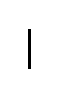
\begin{tikzpicture}%
         \draw[very thick] (\topx,0) -- (\botx,0.5);%
    \end{tikzpicture}%
}
\newcommand{\nimgame}[1]{%
    \begin{center}%
        \def\listofgames{#1}%
        \foreach \heap in \listofgames {%
            \foreach \heapindex in {1, ..., \heap} {%
                \drawnimstick\hspace{0.5mm}%
            }%
            \hspace{10mm}%
        }%
    \end{center}%
}
%</nimsticks>
%\fi
